
\chapter{How to Use CugThesis}

For a thesis based on CugTehsis, we just focused on contents, e.g., text, figures, references, tables, equations and their cross reference. The other details about this template will be updated on \href{https://www.jianshu.com/p/c9bb775fe0f4}{简书文章: CugTheis使用说明}  。

\subsection{Incert Figure}
\begin{figure} [htbp] 
	\centering
	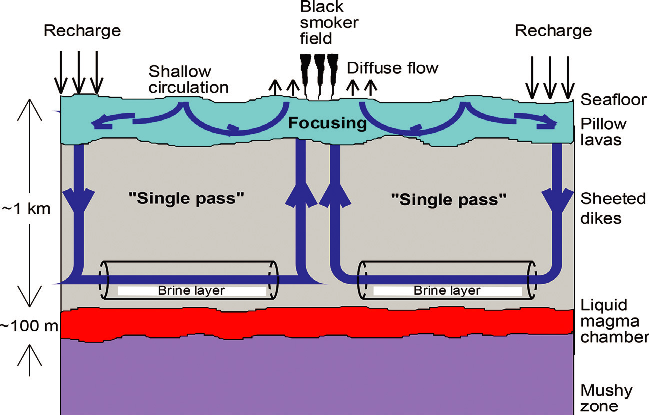
\includegraphics[width=\textwidth ]{SinglePassModel} 
	\caption[Single-Pass Model]{Single Pass Model} 
	\fnote{Diagrammatic sketch of single-pass model, which include recharge zone and discharge zone. The down flow fluid is heated up by deep magmatic heat soource and then phase seperation occurs.} 
	\label{fig:singlepassmodel} 
\end{figure} 

 \autoref{fig:singlepassmodel} is a single figure \footnote{This is a foot note:note that reference citation}
  \citep{andersen2017faulting}。Each figure has a labe, caption and an alternative short caption。
 

\begin{figure} [htbp]
	\centering%
	\subcaptionbox{Color CUG logo\label{fig:cug1} }  
	{\includegraphics[height=0.3\textwidth]{CUG_Logo1} } 
	\hspace{0.01\textwidth} 
	\subcaptionbox{Wechat \label{fig:weixin} }  
	{\includegraphics[height=0.3\textwidth]{weixingongzhong} } 
		\hspace{0.01\textwidth} 
	\subcaptionbox{White-Black CUG logo\label{fig:cug2} }  
	{\includegraphics[height=0.3\textwidth]{CUG_Logo2} } 
	\caption{Three-column Figure} 
	\label{fig:figure_3col} 
\end{figure} 

\autoref{fig:figure_3col} is a three-column figure, it has a main caption and three sub-captions and sub-numbers。For instance, following wechat \ref{fig:weixin} to get much more academic resoources. 


\subsection{Table}

Three-line table

\begin{table}[htbp]
	\centering
	\caption{Symbols and Values}
	\label{tab:symbols_values}
	\begin{tabular}{cccc}
		\toprule 
		Symbol & Definition & Value &Unit \\
		\midrule
		$\vec{g}$ & Gravitational acceleration & 9.8 & $m/s^2$ \\
		$\rho_f$ & Density of water & 1.0 & $kg/m^3$ \\
		\bottomrule
	\end{tabular}
\end{table}

\autoref{tab:symbols_values} is a three-line table with label and caption。

\subsection{Equations}

Inline equation $E=MC^2$,the following is a independent equation,

\begin{equation}
\left( {\phi {\rho _f}{c_{pf}} + \left( {1 - \phi } \right){\rho _r}{c_{pr}}} \right)\frac{{\partial T}}{{\partial t}} = \nabla  \cdot \left( {{K_r}\nabla T} \right) - {\rho _f}{c_{pf}}\vec v \cdot \nabla T + \frac{{{\mu _f}}}{k}{\vec v^2} - {\left( {\frac{{\partial \;ln\rho }}{{\partial \;lnT}}} \right)_p}\frac{{Dp}}{{Dt}}
\label{eq:EnergyConservation}
\end{equation}

 \ref{eq:EnergyConservation} represents energy conservation of hydrothermal fluid flow。

\subsection{References}
First cite format:\cite{vehling2018implementation} noted that phase seperation occurs in deep。
The second cite format:there are some research focus on 3-D simulation \citep{coumou2008structure,coumou2006dynamics}。
